\section{Resultados}
\label{sec:resultados}

\subsection{Artefatos entregues}

Ao final do ciclo, as seis provas de conceito estavam implementadas e
demonstráveis de forma independente, conforme a Regra de Ouro: fundação
jogável; laboratório funcional com missão completa; ARIA integrada por adapter;
mundo reativo; laboratório procedural; e o vertical slice com tutorial,
persistência, áudio e epílogo. O material público inclui o código-fonte, a
especificação com requisitos e critérios de aceitação, as capturas de tela
usadas neste artigo e um vídeo de demonstração de 1~min~08~s
(1280$\times$768 a 30~fps) que percorre a missão do POC~2
\citep{lab404repo,lab404video}. O conjunto de scripts do jogo soma cerca de
2.400 linhas de GDScript (contagem bruta de linhas, incluindo comentários) e a
suíte de testes do motor, cerca de 1.300 linhas.

\subsection{Suíte automatizada}

A \autoref{tab:verificacoes} detalha as verificações por POC. No total, 210 a
211 verificações do motor mais 16 testes do adapter, todas aprovadas na
execução de referência. A variação de uma verificação no POC~3 é esperada: com
o adapter no ar, um dos casos de \emph{fallback} dá lugar à validação da
resposta real do modelo.

\begin{table}[H]
\centering
\caption{Verificações automatizadas por prova de conceito (suíte \emph{headless}, execução de referência de 2026-09-10).}
\label{tab:verificacoes}
\begin{tabular}{@{}l >{\raggedright\arraybackslash}p{96mm} r@{}}
\toprule
POC & Escopo validado & Verificações \\
\midrule
1 & Fundação jogável: input semântico, movimento, câmera, pausa, HUD, diagnóstico de input & 77 \\
2 & Laboratório funcional: interação, inventário, porta, missão, sala modelada & 34 \\
3 & ARIA: adapter, terminal, timeout, validação de intenção, fallback & 25--26 \\
4 & Mundo inteligente: NPC, luzes por energia, tom da ARIA, memória em camadas & 21 \\
5 & Laboratório procedural: determinismo por semente, conectividade entre módulos & 23 \\
6 & Vertical slice: tutorial, missão completa, save/load, áudio, epílogo & 30 \\
Adapter & API de ARIA (Python): contratos, validação, erros e limites & 16 \\
\midrule
Total & & 210--211 + 16 \\
\bottomrule
\end{tabular}
\end{table}

\begin{figure}[H]
\centering
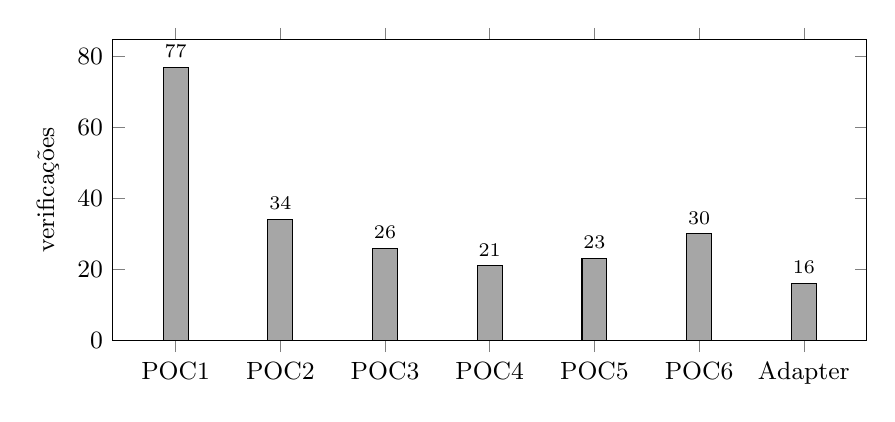
\begin{tikzpicture}
\begin{axis}[
  ybar,
  width=0.92\textwidth,
  height=5.4cm,
  bar width=9pt,
  ymin=0,
  ylabel={verificações},
  symbolic x coords={POC1,POC2,POC3,POC4,POC5,POC6,Adapter},
  xtick=data,
  nodes near coords,
  every node near coord/.append style={font=\scriptsize},
  tick label style={font=\small},
  label style={font=\small},
]
\addplot[fill=black!35] coordinates {
  (POC1,77) (POC2,34) (POC3,26) (POC4,21) (POC5,23) (POC6,30) (Adapter,16)
};
\end{axis}
\end{tikzpicture}
\caption{Distribuição das verificações automatizadas por etapa do projeto.}
\label{fig:verificacoes}
\end{figure}

\subsection{Cena 3D e desempenho}

A sala do laboratório foi exportada em um único arquivo GLB com 342 nós, 37
materiais e 35 objetos de colisão embutidos, totalizando 1.018,7~KB; o emissivo
dos materiais usa a extensão \texttt{KHR\_materials\_emissive\_strength}, o que
permitiu acender telas e sinalizações sem estourar o branco no renderizador
compatível. A \autoref{fig:sala} mostra o resultado em jogo. O desempenho
medido foi de 60~FPS limitados por \emph{vsync} a 1280$\times$720 na GPU
integrada, inclusive após o detalhamento da cena (342 objetos e 34 elementos
de iluminação/letreiros), mantendo o critério NFR-001. Métricas de tempo de
quadro por percentil não foram coletadas
[MEDIÇÃO DE FRAME TIME NÃO REALIZADA].

\begin{figure}[H]
\centering

\includegraphics[width=0.92\textwidth]{sala-energizada.png}
\caption{Vista da sala do Laboratório 404 com a energia restaurada: luminárias do teto acesas, câmera de segurança ativa, porta B1 liberada e letreiros das estações. Captura do jogo em 1280$\times$720 (fonte: material do projeto).}
\label{fig:sala}
\end{figure}

\subsection{Conversa com ARIA}

O critério de aceitação central --- receber uma resposta útil ou um
\emph{fallback} em tempo limitado, sem travar o jogo --- foi validado em três
contextos com o modelo local \texttt{llama3.1:8b}
(\autoref{tab:latencia}). As latências ficaram entre 12,9~s e 22,0~s; a
partida fria é o pior caso, e o teste no jogo (\autoref{fig:terminal}) passou
5 de 5 verificações de integração. O modelo-alvo declarado na especificação,
\texttt{llama3.2:3b}, não estava instalado no ambiente de referência, de modo
que os números representam o desempenho com um modelo maior e mais lento ---
ou seja, são um limite superior conservador para o alvo. Com o adapter ou o
modelo fora do ar, o jogo responde com texto de \emph{fallback} e intenção
\texttt{NONE}, conforme projetado (CA-009).

\begin{table}[H]
\centering
\caption{Latências medidas da conversa com ARIA usando modelo local \texttt{llama3.1:8b}.}
\label{tab:latencia}
\begin{tabular}{@{}>{\raggedright\arraybackslash}p{64mm} l r >{\raggedright\arraybackslash}p{36mm}@{}}
\toprule
Contexto & Intenção & Latência & Observação \\
\midrule
Chamada direta ao adapter (partida fria) & DIAGNOSE & 22,0 s & confiança 0,9 \\
Terminal de ARIA no jogo & STATUS & 16,1 s & captura em \texttt{docs/images} \\
Cliente no jogo (teste ao vivo) & HINT & 12,9 s & 5 de 5 verificações \\
\bottomrule
\end{tabular}
\end{table}

\begin{figure}[H]
\centering

\includegraphics[width=0.92\textwidth]{aria-terminal.png}
\caption{Terminal de ARIA no jogo: a pergunta do jogador e a resposta do modelo local (latência de 16,1~s, intenção \texttt{STATUS}). Fonte: material do projeto.}
\label{fig:terminal}
\end{figure}
